\chapter{MIT bag model}

Smoothly introduce concepts in intro and some other concepts (like bag constant and strange matter hypothesis)

A classic

Treat two and three flavor versions together: they are very similar.
Therefore write $(s)$.

Constant masses $m_u = \ldots$ etc.

QCD Lagrangian when neglecting gluons completely:
\begin{equation}
	\lagr = \bar{q} (i \slashed\partial + \mu \gamma^0 - m) q
	      = \sum_{c=1}^{N_c} \sum_{f=\{u,d,(s)\}} \bar{q}_{f,c} (i \slashed\partial + \mu_f \gamma^0 - m_f) q_{f,c}
\label{eq:mit:lagrangian}
\end{equation}

\section{Partition function, grand potential and equation of state}

With the Euclidean version of the Lagrangian density \eqref{eq:mit:lagrangian},
the partition function \eqref{eq:master_intro:partition_function} reads
\begin{equation}
	Z(V, T, \mu_i) = \prod_{c=1}^{N_c} \prod_{f=\{u,d,(s)\}} \oint_- \pathintdif \bar{q}_{f,c} \oint_- \pathintdif q_{f,c} \exp \bigg\{ \int_0^\beta \dif \tau \int_V \dif^3 x \lagr_E [q_{f,c},\bar{q}_{f,c}] \bigg\} .
\end{equation}
It decouples into a product of path integrals \eqref{eq:tft:dirac_partition_function_first} that we encountered back in \cref{chap:tft}.
There we simplified these path integrals to the form \eqref{eq:tft:dirac_partition_function} for arbitrary temperature.
Then we neglected the vacuum contribution from the first term and calculated it explicitly in the zero-temperature approximation,
arriving at the pressure \eqref{eq:nstars:pressure_zeroT} that is related to the grand potential density \eqref{eq:master_intro:grand_potential} by a simple sign flip.
Adding a background of free electrons and reinstating the Fermi momenta $p_f = \sqrt{\mu_f^2-m_f^2}$ for each particle,
we can then write the grand potential density as
\begin{equation}
	\Omega(\mu_u,\mu_d,\mu_s,\mu_e) = -\smashoperator{\sum_{\vphantom{\big|} f=\{3u,3d,(3s),e\}}} \frac{1}{24 \pi^2} \left[ \left( 2 \mu_f^2 - 5 m_f^2 \right) \mu_f \sqrt{\mu_f^2 - m_f^2} + 3 m_f^4 \asinh \left( \sqrt{\frac{\mu_{\smash{f}}^2}{m_f^2}-1} \right) \right] .
\label{eq:mit:grand_potential}
\end{equation}
Our notation below the flavor sum means that the quark terms are multiplied by $N_c=3$,
but the electron contribution is not.
The corresponding quark and electron densities \eqref{eq:master_intro:densities} are
\begin{equation}
	n_f = -\pdv{\Omega}{\mu_f} = \frac{N_c}{3 \pi^2} \Big( \mu_f^2 - m_f^2 \Big)^{\frac32}
	\text{ for $f \in \{u,d,(s)\}$}
	\quad \text{and} \quad
	n_e = -\pdv{\Omega}{\mu_e} = \frac{  1}{3 \pi^2} \Big( \mu_e^2 - m_e^2 \Big)^{\frac32},
\label{eq:mit:particle_densities}%
\end{equation}
and the pressure \eqref{eq:master_intro:pressure} and energy density \eqref{eq:master_intro:energy_density} follow.

We now see explicitly that the grand potential and hence the pressure and energy density are functions of the four chemical potentials $\mu_u$, $\mu_d$, $\mu_s$ and $\mu_e$.
As explained in \cref{sec:master_intro:tft},
we reduce them to only one independent chemical potential with the three constraints \eqref{eq:lsm:chemical_equilibrium} and \eqref{eq:lsm:charge_neutrality} --
and take this to be the quark chemical potential $\mu_Q$ defined in equation \eqref{eq:master_intro:chemical_potentials_transformed}.
With the densities \eqref{eq:mit:particle_densities} and for a given value of $\mu_Q$,
we must then find the electron chemical potential $\mu_e$ that solves
\TODO{create and refer to table with quark properties: name, electric charges, two masses}
\begin{equation}
	2 \Big[\mu_u^2-m_u^2\Big]^\frac32
	- \Big[(\mu_u+\mu_e)^2-m_d^2\Big]^\frac32 
	- \Big[(\mu_u+\mu_e)^2-m_s^2\Big]^\frac32 
	- \Big[\mu_e^2-m_e^2\Big]^\frac32 = 0,
\label{eq:mit:charge_neutrality_explicit}
\end{equation}
after which the two remaining chemical potentials are given by the chemical equilibrium constraint \eqref{eq:lsm:chemical_equilibrium}. 
Elimination of the three chemical potentials yields two functions $P(\mu_u)$ and $\epsilon(\mu_u)$,
and the former can finally be inverted to yield the equation of state $\epsilon(P)$.
Using the program in \TODO{ref appendix},
we obtain the chemical potentials, densities and equation of state shown in \cref{fig:mit:eos}.

\begin{figure}
\centering
\tikzsetnextfilename{mit-eos}
\begin{tikzpicture}
\tikzset{declare function={
	muQ(\muu,\mud)=(\muu+\mud)/2;
	muu(\muQ)=2/(1+2^(1/3))*\muQ;
	mud(\muQ)=2/(1+2^(-1/3))*\muQ;
	mue(\muQ)=2*(2^(1/3)-1)/(2^(1/3)+1)*\muQ;
	nq(\mu)=3/(3*pi^2)*(\mu)^3;
	ne(\mu)=1/(3*pi^2)*(\mu)^3;
	nconv=1.29619e-7;
}};
\begin{groupplot}[
	group style={group size={1 by 3}, vertical sep=2.0cm},
	width=13cm, height=7cm,
	extra tick style={grid=major, grid style={dashed}},
	minor tick num=9,
]
\nextgroupplot[
	xlabel={$\mu_Q \, / \, \si{\mega\electronvolt}$}, ylabel={$\mu_i \, / \, \si{\mega\electronvolt}$},
	%xmin=0, xmax=600, ymax=500, xtick distance=100, ytick distance=100, minor x tick num=9,
	xmin=0, xmax=1000, xtick distance=100, minor x tick num=9,
	ymin=0, ymax=1000, ytick distance=100, 
	%ymax=600, 
	title={\subcaption{\label{fig:mit:eos-parametrization}Parametrization of solutions}},
	legend cell align=right, legend pos=north west,
];
% fake legend
\addplot+ [black, solid, opacity=0.3] {-100}; \addlegendentry{$N_f=2$};
\addplot+ [black, solid, opacity=0.8] {-100}; \addlegendentry{$N_f=3$};
\addplot+ [red, solid, opacity=1.0] {-100}; \addlegendentry{$i=u$};
\addplot+ [darkgreen, solid, opacity=1.0] {-100}; \addlegendentry{$i=d$};
\addplot+ [purple, solid, opacity=1.0] {-100}; \addlegendentry{$i=s$};
\addplot+ [blue, solid, opacity=1.0] {-100}; \addlegendentry{$i=e$};

% 2-flavor
\addplot+ [red,       solid,  opacity=0.3] table [x expr={muQ(\thisrow{muu},\thisrow{mud})}, y=muu] {../code/data/MIT2F/eos_sigma_800.dat};
\addplot+ [darkgreen, solid,  opacity=0.3] table [x expr={muQ(\thisrow{muu},\thisrow{mud})}, y=mud] {../code/data/MIT2F/eos_sigma_800.dat};
\addplot+ [blue,      solid,  opacity=0.3] table [x expr={muQ(\thisrow{muu},\thisrow{mud})}, y=mue] {../code/data/MIT2F/eos_sigma_800.dat};

% 3-flavor
\addplot+ [red,       solid,  opacity=0.8] table [x expr={muQ(\thisrow{muu},\thisrow{mud})}, y=muu] {../code/data/MIT3F/eos_sigma_800.dat};
\addplot+ [darkgreen, solid,  opacity=0.8] table [x expr={muQ(\thisrow{muu},\thisrow{mud})}, y=mud] {../code/data/MIT3F/eos_sigma_800.dat};
\addplot+ [purple,    dashed, opacity=0.8] table [x expr={muQ(\thisrow{muu},\thisrow{mud})}, y=mus] {../code/data/MIT3F/eos_sigma_800.dat};
\addplot+ [blue,      solid,  opacity=0.8] table [x expr={muQ(\thisrow{muu},\thisrow{mud})}, y=mue] {../code/data/MIT3F/eos_sigma_800.dat};

\nextgroupplot[
	xlabel={$\mu_Q \, / \, \si{\mega\electronvolt}$}, ylabel={$n_i \, / \, (1/\si{\femto\meter\cubed})$},
	xmin=0, xmax=1000, xtick distance=100, minor x tick num=9,
	ymin=-0.2, ymax=10.0, ytick distance=1.0, minor y tick num=4, restrict y to domain=-10:10,
	title={\subcaption{\label{fig:mit:eos-density}Particle number densities}},
	legend cell align=right, legend pos=north west,
];
% fake legend
\addplot+ [black, solid, opacity=0.3] {-10}; \addlegendentry{$N_f=2$};
\addplot+ [black, solid, opacity=0.8] {-10}; \addlegendentry{$N_f=3$};
\addplot+ [red, solid, opacity=1.0] {-10}; \addlegendentry{$i=u$};
\addplot+ [darkgreen, solid, opacity=1.0] {-10}; \addlegendentry{$i=d$};
\addplot+ [purple, solid, opacity=1.0] {-10}; \addlegendentry{$i=s$};
\addplot+ [blue, solid, opacity=1.0] {-10}; \addlegendentry{$i=e$};

% 2-flavor
\addplot+ [red,       solid, opacity=0.3] table [x expr={muQ(\thisrow{muu},\thisrow{mud})}, y=nu] {../code/data/MIT2F/eos_sigma_800.dat};
\addplot+ [darkgreen, solid, opacity=0.3] table [x expr={muQ(\thisrow{muu},\thisrow{mud})}, y=nd] {../code/data/MIT2F/eos_sigma_800.dat};
\addplot+ [blue,      solid, opacity=0.3] table [x expr={muQ(\thisrow{muu},\thisrow{mud})}, y=ne] {../code/data/MIT2F/eos_sigma_800.dat};

% 3-flavor
\addplot+ [red,       solid, opacity=0.8] table [x expr={muQ(\thisrow{muu},\thisrow{mud})}, y=nu] {../code/data/MIT3F/eos_sigma_800.dat};
\addplot+ [darkgreen, solid, opacity=0.8] table [x expr={muQ(\thisrow{muu},\thisrow{mud})}, y=nd] {../code/data/MIT3F/eos_sigma_800.dat};
\addplot+ [purple,    solid, opacity=0.8] table [x expr={muQ(\thisrow{muu},\thisrow{mud})}, y=ns] {../code/data/MIT3F/eos_sigma_800.dat};
\addplot+ [blue,      solid, opacity=0.8] table [x expr={muQ(\thisrow{muu},\thisrow{mud})}, y=ne] {../code/data/MIT3F/eos_sigma_800.dat};

\nextgroupplot[
	xlabel={$P        \, / \, (\si{\giga\electronvolt\per\femto\meter\cubed})$},
	ylabel={$\epsilon \, / \, (\si{\giga\electronvolt\per\femto\meter\cubed})$},
	xmin=0, xmax=0.30, ymin=0, ymax=1.0, xtick distance=0.10, minor x tick num=9, ytick distance=0.5, minor y tick num=4, restrict y to domain=-1:+1,
	title={\subcaption{\label{fig:mit:eos-eos}Equation of state}},
	legend cell align=left, legend pos=north west,
];
\addplot+ [black, solid, opacity=0.3] table [x=P,y=epsilon] {../code/data/MIT2F/eos_sigma_800.dat}; \addlegendentry{$N_f=2$};
\addplot+ [black, solid, opacity=0.8] table [x=P,y=epsilon] {../code/data/MIT3F/eos_sigma_800.dat}; \addlegendentry{$N_f=3$};
\end{groupplot}
\end{tikzpicture}
\caption{\label{fig:mit:eos}%
Properties of electrically charge neutral two-flavor (weak lines) and three-flavor (strong lines) MIT bag model quark matter in $\beta$-equilibrium parametrized by the common quark chemical potential $\mu_Q = (\mu_u+\mu_d)/2$.
Upper panel \subref{fig:mit:eos-parametrization} shows the relations between chemical potentials due to the constraints \eqref{eq:lsm:chemical_equilibrium} and \eqref{eq:lsm:charge_neutrality},
middle panel \subref{fig:mit:eos-density} the corresponding particle number densities \eqref{eq:mit:particle_densities} and
lower panel \subref{fig:mit:eos-eos} the resulting equation of state.
}
\end{figure}

\subsubsection{Ultra-relativistic limit}

Note that the electron density is very small, but nonzero,
and that the chemical potentials and equation of state seems to converge to a simple linear form in the ultra-relativistic limit $\mu_i \gg m_i$.
In fact, we can find analytical expressions for the chemical potentials, densities and equation of state in the limit $m_i \rightarrow 0$.
The grand potential \eqref{eq:mit:grand_potential} then reduces to
\begin{equation}
	\Omega(\mu_u, \mu_d, \mu_e) = -\frac{N_c \mu_u^4}{12 \pi^2} - \frac{N_c \mu_d^4}{12 \pi^2} - \frac{N_c \mu_s^4}{12 \pi^2} - \frac{\mu_e^4}{12 \pi^2},
\label{eq:mit:grand_potential_massless}
\end{equation}
while the densities \eqref{eq:mit:particle_densities} become
\begin{equation}
	n_f = -\pdv{\Omega}{\mu_f} = \frac{N_c \mu_f^3}{3 \pi^2}
	\text{ for $f \in \{u,d,(s)\}$}
	\quad \text{and} \quad
	n_e = -\pdv{\Omega}{\mu_e} = \frac{    \mu_e^3}{3 \pi^2}.
\label{eq:lsm:densities_massless}
\end{equation}
\emph{Regardless} of the relations between the chemical potentials,
the equation of state is then
\begin{equation}
	\epsilon = -P + \sum_i \mu_i n_i
	         = -P + \frac{1}{3 \pi^2} \Big(N_c \mu_u^4 + N_c \mu_d^4 + N_c \mu_s^4 + \mu_e^4\Big)
	         = -P - 4 \Omega 
	         = -P + 4 P 
	         = 3 P .
\end{equation}
We can also find approximate analytical relations between the chemical potentials in the ultra-relativistic limit
if we also neglect the electron density in the charge neutrality condition \eqref{eq:mit:charge_neutrality_explicit},
motivated by its very low value $n_e \ll n_u < n_d$ in the numerical solution.
In the two-flavor case, this simplifies the condition to $n_d = 2 n_u$ with the solution $\mu_d = 2^{1/3} \mu_u$.
According to the $\beta$-equilibrium condition \eqref{eq:lsm:minsys_equilibrium},
the chemical potential of the electrons is then $\mu_e = \mu_d - \mu_u = (2^{1/3}-1) \mu_u$
and corresponds to the density $n_e = (2^{1/3}-1)^3 n_u / N_c = 0.006 \, n_u \ll n_u < n_d$,
showing that our approximation of neglecting the electron density is self-consistent.
Expressing the chemical potentials in terms of the common quark chemical potential \eqref{eq:master_intro:chemical_potentials_transformed},
we then have
\begin{equation}
	\mu_u = \underbrace{\frac{2}{1+2^{1/3}}}_{0.88} \mu_Q , \quad
	\mu_d = \underbrace{\frac{2}{1+2^{-1/3}}}_{1.12} \mu_Q \quad \text{and} \quad
	\mu_e = \underbrace{2 \frac{2^{1/3}-1}{2^{1/3}+1}}_{0.29} \mu_Q
	\qquad (N_f = 2) .
\label{eq:mit:chemical_potentials_massless_2f}
\end{equation}
With three flavors, the charge neutrality condition \eqref{eq:mit:charge_neutrality_explicit} becomes $2 n_u - n_d - n_s = 0$
and has the very simple solution $n_u = n_d = n_s$ and $\mu_u = \mu_d = \mu_s$.
As $\mu_e = \mu_d - \mu_u = 0$, neglecting the electron contribution is exact in this case.
In terms of the common quark chemical potential, the particle chemical potentials are then
\begin{equation}
	\mu_u = \mu_d = \mu_s = \mu_Q
	\qquad \text{and} \qquad
	\mu_e = 0
	\qquad (N_f = 3) .
\label{eq:mit:chemical_potentials_massless_3f}
\end{equation}
Upon inspection we see that the solutions in \cref{fig:mit:eos} are very close to these ultra-relativistic expressions as $\mu_i \rightarrow \infty$.
This verifies our numerical calculations.

\section{Bag constant and strange matter hypothesis}

Pressure above is normalized so that it vanishes for $\mu < m$.
This is called the vacuum because $n = 0$ then.
More generally, it is customary to shift it like $P \rightarrow P - B$ so that $P = -B$ for $\mu < m$,
causing $\epsilon = +B$.
$B$ is called the bag constant.
\TODO{explain stuff about bag constant}

\section{Mass-radius solutions}

\TODO{old stuff below}

To model quark matter and the effect of these two properties,
physicists have come up with various \textbf{bag models}.
As illustrated in \cref{fig:lsm:confinement}, these models split the medium of the physical vacuum state into two phases.
The \emph{normal phase} is the background phase in which quarks are forbidden to exist -- remains of the non-confining medium that existed before the separation into two phases.
On top of the background, bubbles of \emph{hadron phase} are created inside which colorless combinations of quarks are confined.
Mathematically, the confinement is implemented by adding a bag constant $B$ to the grand potential density $\Omega$ of the quarks assumed to live inside the hadronic bubbles.
The bag constant is therefore defined as the energy difference between the hadronic phase and the normal phase,
and creating a hadronic bubble of volume $V$ costs the energy $B V$.
A positive bag constant gives a negative contribution to the pressure $P = -\Omega$,
hence confining the contents of the bag with an external pressure from the surrounding medium in the normal phase.

The \textbf{MIT bag model} is the simplest example.
Consider a star composed of up, down and strange quarks in the zero-temperature and massless approximation.
According to what we learned in \TODO{ref 4.12} and \eqref{eq:nstars:ur_eos}, the grand potential ``before bagging'' is
Pressure
\begin{equation}
	P(\mu) = \smashoperator{\sum_{f=\{u,d,s\}}} \frac{N_c \mu_f^4}{12 \pi^2}
	\qquad \text{and} \qquad
	\epsilon(\mu) = -P(\mu) + \smashoperator{\sum_{f=\{u,d,s\}}} \frac{N_c \mu_f^4}{3 \pi^2}.
\end{equation}
After ``bagging'' the quarks with a bag constant $B$,
\begin{equation}
\begin{split}
	P(\mu,B) = P(\mu) - B, \\
	\epsilon(\mu,B) = -P(\mu,B) + \smashoperator{\sum_{f=\{u,d,s\}}} \frac{N_c \mu_f^4}{3 \pi^2}.
	                = -P(\mu,B) + 4 (P(\mu,B) + B) = 4 P(\mu,B) + 4 B.
\end{split}
\end{equation}
The energy density and equation of state is then
\begin{equation}
	\epsilon(P) = -P + \sum_f \mu_f n_f = -P + \sum_f \frac{N_c \mu_f^4}{3 \pi^2} = -P + 4P = 3P
\end{equation}
To ``bag'' the quarks, the idea is 

In the early days of high density and temperature, the universe likely passed through a deconfined quark matter phase.
Today, matter is accreting by nuclear fusion in stars towards iron-56, seemingly representing the ground state of nuclear matter.
However, \cite{ref:strange_hypothesis_bodmer} and \cite{ref:strange_hypothesis_witten} has hypothesized that this state of matter is only \emph{metastable}.
Their \textbf{strange matter hypothesis} claims that the true ground state of nuclear matter is that of three-flavor matter consisting of up, down and strange quarks

\TODO{rewrite?}
We can use the presumed stability of two-flavor and three-flavor quark matter to determine a range of acceptable windows for the bag constant $B$.
Per baryon, iron-56 has an energy of $E/N_B = \epsilon/n_B = \SI{930}{\mega\electronvolt}$,
so if $\epsilon_2$ and $\epsilon_3$ are the energy densities of two-flavor and three-flavor quark matter,
we determine the bag constant $B$ such that
\TODO{at zero pressure?}
\begin{equation}
	\frac{\epsilon_3(0)}{n_B} < \SI{930}{\mega\electronvolt} < \frac{\epsilon_2(0)}{n_B} .
\label{eq:lsm:bag_stability}
\end{equation}
Only the two-flavor bound has been observed,
while the three-flavor bound is a quite reckless assumption that should certainly be taken with a grain of salt.
It will, however, be very useful to have \emph{some} bound for the bag constant in order to constrain the parameter space of equations of state later on.

% TODO: start here
\begin{figure}[bh!]
\centering
\tikzsetnextfilename{bag-mass-radius}
\begin{tikzpicture}
\begin{axis}[
	width=15cm, height=12cm,
	xlabel={$R \, / \, \si{\kilo\meter}$}, ylabel={$M \, / \, M_\odot$}, title={Mass-radius diagram for bag-model quark stars }, title style={yshift=2.0cm},
	xmin=0, xmax=15, ymin=0.0, ymax=2.2, xtick distance=1, ytick distance=0.1, minor tick num=9, grid=major,
	point meta=explicit, point meta min=32, point meta max=39,
	colorbar horizontal, colormap name=plasmarev, colorbar style={xlabel=$\log_{10} (P_c \, / \, \si{\pascal})$, xtick distance=1, minor x tick num=9, at={(0.5,1.03)}, anchor=south, xticklabel pos=upper},
	declare function={
		e0 = 4.266500881855304e+37;
	},
	legend pos=north east, legend cell align=right,
]
\tikzset{
	Bpin/.style={gray, sloped, allow upside down=true, rotate=180, yshift=+0.4cm, font=\small},
}
\addplot+ [mesh] table [x=R, y=M, meta expr={log10(\thisrow{P}*e0)}] {../code/data/MIT2F/stars_B14_144.dat}; % node [Bpin, pos=0.920] {$B = (\SI{27}{\mega\electronvolt})^4$};
\addplot+ [mesh] table [x=R, y=M, meta expr={log10(\thisrow{P}*e0)}] {../code/data/MIT2F/stars_B14_163.dat}; % node [Bpin, pos=0.920] {$B = (\SI{27}{\mega\electronvolt})^4$};
\end{axis}
\end{tikzpicture}
\caption{\TODO{MIT bag model 2 and 3 flavors}}
\end{figure}

\TODO{titles}

\TODO{units, $\hbar = c = G = k_B = 1$ or not?}

\TODO{organize project and master thesis together}

\TODO{color confinement, asymptotic freedom, bag models, etc.}
\begin{figure}
\centering
\tikzsetnextfilename{bag-model}
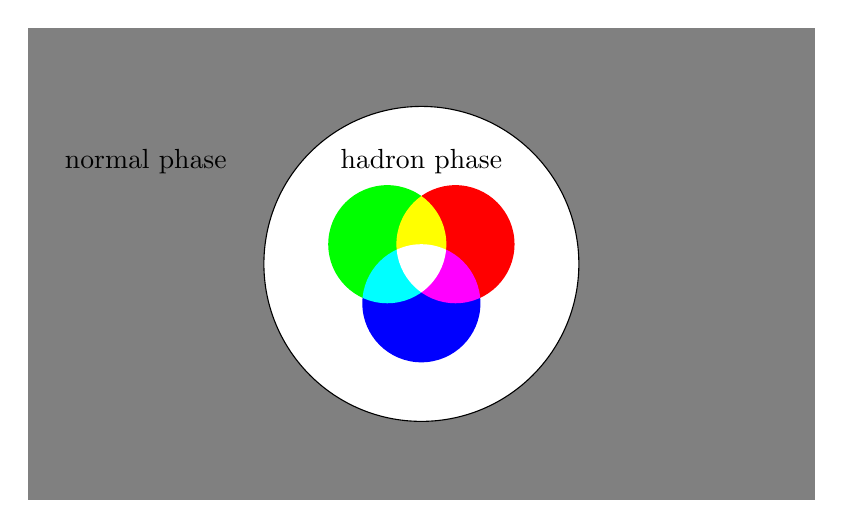
\begin{tikzpicture}
\fill [gray] (-5, -3) rectangle (+5, +3);

\draw [draw=black, fill=white] (0, 0) circle (2);
\begin{scope}[blend group=screen]
	\fill [fill=red]   (30:0.5)  circle (0.75) node {$u$};
	\fill [fill=green] (150:0.5) circle (0.75) node {$d$};
	\fill [fill=blue]  (270:0.5) circle (0.75) node {$s$};
\end{scope}
\node at (90:1.3) {hadron phase};
\node at (-3.5,1.3) {normal phase};
\end{tikzpicture}
\caption{\label{fig:master_intro:confinement}%
	\TODO{create different confinement vs deconfinement figure}
}
\end{figure}
